% Build from this directory:
%   inkscape readable-reality-return.svg --export-type=pdf --export-filename=readable-reality-return.pdf
%   pdflatex -halt-on-error -interaction=nonstopmode Displacement_Of_Origin_reader_edition.tex
%   pdflatex -halt-on-error -interaction=nonstopmode Displacement_Of_Origin_reader_edition.tex
\documentclass[11pt,letterpaper]{article}
\usepackage[letterpaper,margin=0.84in,headheight=22pt,headsep=16pt,footskip=25pt]{geometry}
\usepackage[T1]{fontenc}
\usepackage[utf8]{inputenc}
\usepackage{mathpazo}
\usepackage{microtype}
\usepackage{amsmath,amssymb,mathtools}
\usepackage{graphicx}
\usepackage{xcolor}
\usepackage{fancyhdr}
\usepackage{titlesec}
\usepackage{enumitem}
\usepackage{needspace}
\usepackage[hidelinks]{hyperref}

\definecolor{paper}{RGB}{248,246,240}
\definecolor{ink}{RGB}{25,39,45}
\definecolor{deep}{RGB}{22,72,80}
\definecolor{muted}{RGB}{91,100,103}
\definecolor{rule}{RGB}{183,191,187}
\definecolor{wash}{RGB}{239,243,241}
\definecolor{accent}{RGB}{161,111,61}
\pagecolor{paper}
\color{ink}
\hypersetup{
  pdftitle={The Displacement of the Origin: Reader Edition},
  pdfauthor={Anthony Vito Coppa},
  pdfsubject={Refusal Wall and Readable Reality Closure},
  pdfkeywords={reference, Difference, memory, return, readable reality, refusal wall}
}

\setlength{\parindent}{0pt}
\setlength{\parskip}{0.62em}
\linespread{1.045}
\setlength{\emergencystretch}{2em}
\allowdisplaybreaks[2]
\setlist[itemize]{leftmargin=1.4em,itemsep=.28em,topsep=.3em}
\setlist[enumerate]{leftmargin=1.65em,itemsep=.35em,topsep=.35em}

\titleformat{\section}{\Large\bfseries\color{deep}}{\thesection.}{.55em}{}
\titleformat{\subsection}{\large\bfseries\color{deep}}{\thesubsection.}{.5em}{}
\titlespacing*{\section}{0pt}{1.55em}{.56em}
\titlespacing*{\subsection}{0pt}{1.05em}{.40em}

\pagestyle{fancy}
\fancyhf{}
\lhead{\small\textsc{Coppalini Architecture}}
\chead{\small\textsc{The Displacement of the Origin}}
\rhead{\small\textsc{Reader Edition}}
\cfoot{\small\textsc{\thepage}}
\renewcommand{\headrulewidth}{.4pt}
\renewcommand{\headrule}{\hbox to\headwidth{\color{rule}\leaders\hrule height \headrulewidth\hfill}}

\newcommand{\src}{\textsc{Source}}
\newcommand{\reader}{\textsc{Reader Edition}}
\newcommand{\eqbox}[1]{%
  \par\vspace{.35em}\noindent
  \fcolorbox{rule}{wash}{\begin{minipage}{.94\linewidth}\centering\vspace{.28em}#1\vspace{.28em}\end{minipage}}%
  \par\vspace{.35em}}
\newcommand{\wallitem}[2]{\item[\textbf{#1}] #2}

\begin{document}
\pagenumbering{gobble}
\begin{titlepage}
\thispagestyle{empty}
\vspace*{.55in}
{\color{deep}\rule{\textwidth}{1.4pt}}\par
\vspace{.34in}
{\small\textsc{Coppalini Architecture / Canonical Reader Edition}}\par
\vspace{.24in}
{\fontsize{34}{39}\selectfont\bfseries\color{ink}The Displacement\\[.04em]of the Origin\par}
\vspace{.22in}
{\Large\color{deep}Refusal Wall \textbar\ Readable Reality Closure\par}
\vspace{.38in}
{\color{rule}\rule{.82\textwidth}{.55pt}}\par
\vspace{.34in}
\begin{minipage}{.86\textwidth}
\large
A readable system fixes a reference, notices Difference, preserves the receipt,
updates only where Difference requires it, and refuses any continuation that
cannot preserve another truthful return.
\end{minipage}\par
\vfill
{\large Anthony Vito Coppa\par}
{\normalsize 24 November 2026\par}
\vspace{.35in}
\begin{minipage}{.88\textwidth}
\small\color{muted}
\textbf{Reader receipt.} Typeset from the canonical source text
\texttt{displacement-of-origin-v0.2.txt}; SHA-256
\texttt{7a4ec67c4d8fe7550746857d0dd5d1c3443bfcb934ee5e54927661609113cfbe}.
The source body begins on the following page. This reader edition adds layout,
navigation, and the existing visual companion only; it adds no new theorem,
physical claim, or interpretive apparatus.
\end{minipage}\par
\vspace{.22in}
{\color{deep}\rule{\textwidth}{1.4pt}}\par
\end{titlepage}

\clearpage
\pagenumbering{arabic}

\section*{Owning Jurisdiction}
\addcontentsline{toc}{section}{Owning Jurisdiction}

The active jurisdiction is the civilization that produced the readers themselves:
the inherited human public field of language, law, science, engineering, records,
institutions, infrastructure, ecology, and shared survival conditions.

No government, laboratory, court, company, model, or AI stands outside that field
merely by exercising authority or technical capacity.

Public duty, evidence, hazard, trust, correction, and stopping are therefore typed
inside a shared civilizational reference before any local office claims authority over them.

\section*{Refusal Wall}
\addcontentsline{toc}{section}{Refusal Wall}

\begin{description}[style=nextline,itemsep=1.05em]
  \wallitem{1. Jurisdiction}{A reusable relation has an owner.
  \eqbox{$\operatorname{Ad}_J(x)\Rightarrow C_J(x)$}
  The owning field is shared civilization and its survivable public conditions.
  No owning constraint: no admission.}

  \wallitem{2. Type}{Typing precedes Gate.
  \eqbox{$\varnothing=\textsc{Untypeable}$.}
  An untyped candidate does not receive a value by force.}

  \wallitem{3. Reference}{Difference requires a fixed reference.
  \eqbox{No reference: no lawful Difference.}
  Silent reference displacement invalidates downstream orientation even when downstream
  calculation remains internally consistent.}

  \wallitem{4. Source and Strength}{A claim cannot carry more authority than its source,
  carrier, conditions, observable, calibration, receipt, and stated boundary.
  \eqbox{No bridge: \textsc{Open}.\quad No calibration: no measured claim.\\
  No source: no promoted relation.\quad No earned strength: no strength inflation.}
  }

  \Needspace{13\baselineskip}
  \wallitem{5. Memory}{Return does not erase the path.
  A recognized form may return while its address advances.
  \eqbox{same read $\neq$ same occurrence}
  Memory retains the Difference required to distinguish them.}

  \wallitem{6. Gate}{Technical possibility is not admissibility.
  Gate acts only on typed candidates. A continuation that violates its governing constraint
  is refused even when it can be executed.}

  \wallitem{7. Survival}{Another truthful lawful continuation must remain available.
  If continuation destroys the condition required for another lawful read, stop.}

  \wallitem{8. Residual}{Completion means the required relation fits at the declared resolution.
  \eqbox{$\varepsilon_{\mathrm{drop}}=0\qquad
  \varepsilon_{\mathrm{add}}=0\qquad
  \varepsilon_{\mathrm{strength}}=0$}
  Anything unresolved remains \textsc{Open}.}
\end{description}

\section*{Exact Closure}
\addcontentsline{toc}{section}{Exact Closure}

\subsection*{I. Root}
\begin{align*}
Q&=\begin{bmatrix}1&1\\1&0\end{bmatrix},
&\Omega&=\begin{bmatrix}0&1\\-1&0\end{bmatrix},\\
G&=[Q,\Omega]=\begin{bmatrix}-2&1\\1&2\end{bmatrix},
&H&=G/\sqrt5,\\[.3em]
Q^2&=Q+I,
&\Omega^2&=-I,\\
G^2&=5I,
&H^2&=I.
\end{align*}

Recurrence, turn, metric Difference, and mirror close on one two-dimensional carrier.

\subsection*{II. Return \textbar\ Memory \textbar\ Transport}
Return = recognizable form.\par
Memory = retained Difference.\par
Transport = addressed change.

A quotient may return while its lift advances:
\eqbox{$q(\xi+\varpi)=q(\xi)\qquad\xi+\varpi\neq\xi$}

The read returns.\par
The occurrence does not disappear.

\begin{figure}[htbp]
  \centering
  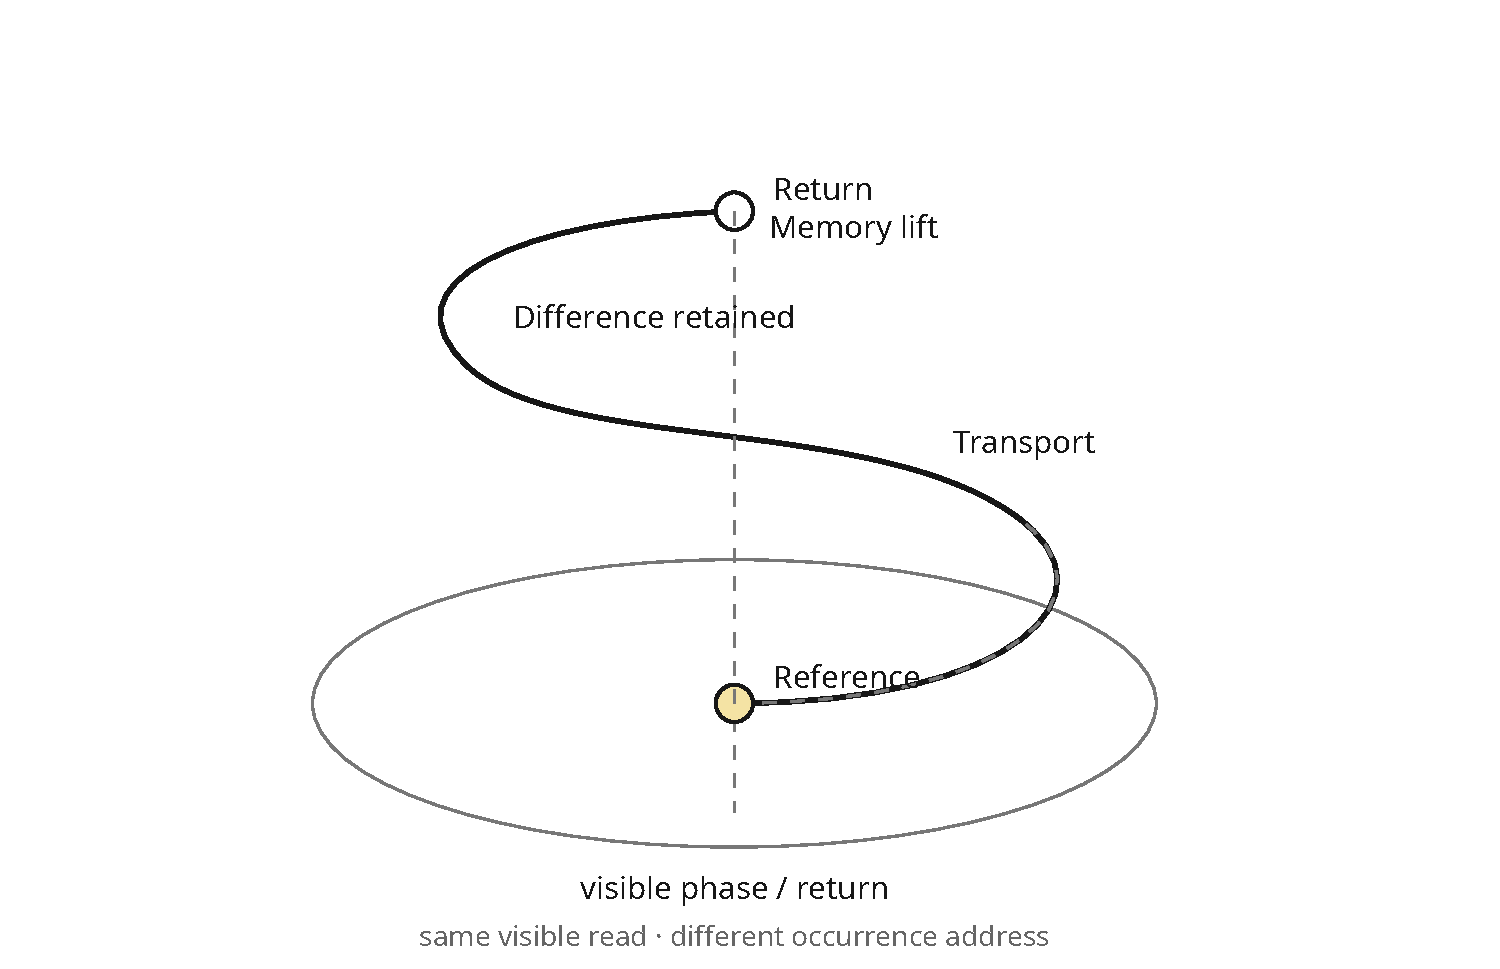
\includegraphics[width=.88\linewidth]{readable-reality-return.pdf}
  \caption{Return with retained memory lift: the visible phase returns while the occurrence address advances.}
\end{figure}

\subsection*{III. Eight Addresses \textbar\ Twenty-Eight Relations \textbar\ Seven Reads}
\begin{align*}
A_8&=\{\infty\}\sqcup\mathbb Z_7,\\
M_r&=\bigl\{\{\infty,r\}\bigr\}\cup\bigl\{\{r+j,r-j\}:j=1,2,3\bigr\},\\
E(K_8)&=\bigsqcup_{r\in\mathbb Z_7}M_r,\qquad 28=7\times4.
\end{align*}

Every finite pair $\{a,b\}$ determines its own midpoint and offset:
\eqbox{$r=4(a+b)\qquad j=4(a-b)\pmod 7$}

because $2$ is invertible modulo $7$.

The partition is not an interpretation placed on the wheel. It is the pair structure
of the declared eight-address carrier.

\subsection*{IV. Four Dual Forms}
\begin{center}
\begin{tabular}{c@{\qquad\qquad}c}
Gravity \textbar\ Light & Memory \textbar\ Motion\\[.35em]
Time \textbar\ Scope & Horizon \textbar\ Silence\\[.8em]
Interval \textbar\ null relation & Return \textbar\ transport\\[.35em]
Phase \textbar\ directional read & Viability boundary \textbar\ completed fit
\end{tabular}
\end{center}

\subsection*{V. Eight Operational Offices}
\begin{center}
\begin{tabular}{rl}
Motion: & Orient \textbar\ Transport\\
Gravity: & Bound \textbar\ Regulate\\
Light: & Cut \textbar\ Read\\
Memory: & Couple \textbar\ Return
\end{tabular}
\end{center}

The two registries remain separately typed.

\subsection*{VI. Two-Reference Mirror}
Reader A fixes reference $a$ and orientation $\sigma_A$.\par
Reader B fixes reference $b$ and orientation $\sigma_B$.

The exchanged coordinate is
\eqbox{$\lambda'=b-\sigma_A\sigma_B(\lambda-a)$.}

When the orientations agree,
\eqbox{$\lambda'=a+b-\lambda$.}

Neither reader is permitted to invent the other's reference. The relation retains both receipts.

My reference belongs to me.\par
Your reference belongs to you.\par
Difference belongs to the relation.\par
Coincidence, if present, is a result.

\subsection*{VII. Horizon \textbar\ Silence}
Let $V$ be the viable region.
\eqbox{$\theta(x)=1\ \text{iff}\ x\in V\qquad H_{\mathrm{hor}}=\partial V$}

Horizon is the boundary of lawful continuation.\par
Silence is completed fit at the present reader resolution.

\clearpage
\section*{Refusal Wall, Fully Compressed}
\addcontentsline{toc}{section}{Refusal Wall, Fully Compressed}

\begin{center}
\large\bfseries\color{deep}
FIX JURISDICTION.\\
FIX REFERENCE.\\
TYPE BEFORE GATE.\\
READ DIFFERENCE.\\
RETAIN MEMORY.\\
UPDATE ONLY WHEN REQUIRED.\\
REFUSE UNSOURCED STRENGTH.\\
STOP AT THE HORIZON.\\
RETURN WITHOUT ERASING THE PATH.
\end{center}

\section*{One-Line Closure}
\addcontentsline{toc}{section}{One-Line Closure}
\eqbox{$\displaystyle\text{Reference}\ \longrightarrow\ \text{Difference}\ \longrightarrow\ \text{Memory}\ \longrightarrow\ \text{Return}\ \longrightarrow\ \text{lawful continuation}.$}

Anything missing from that chain remains \textsc{Open}.

\section*{Readable Reality}
\addcontentsline{toc}{section}{Readable Reality}

Readable reality is the condition in which a relation can still answer:
\begin{itemize}
  \item Where is the reference?
  \item What changed?
  \item What stayed invariant?
  \item Who or what authorizes the relation?
  \item What receipt preserves the occurrence?
  \item What would require correction?
  \item What would require stopping?
  \item Can another truthful continuation still occur?
\end{itemize}

If those answers cannot be recovered, calculation may continue, but orientation has been lost.

\textbf{The displacement of the origin is therefore minimal:}\par
A system can be locally correct and globally wrong when it forgets what its calculations are relative to.

\Needspace{9\baselineskip}
\textbf{The repair is equally minimal:}
\begin{quote}
Return to the reference.\par
Read the Difference.\par
Preserve the receipt.\par
Correct only what changed.\par
Continue only while another truthful return remains possible.
\end{quote}

\vspace{1.2em}
\begin{center}
\color{rule}\rule{.76\textwidth}{.45pt}\par\vspace{.7em}
\small\color{muted}
Canonical body: \texttt{displacement-of-origin-v0.2.txt}\par
Source SHA-256: \texttt{7a4ec67c4d8fe7550746857d0dd5d1c3443bfcb934ee5e54927661609113cfbe}\par
Visual companion SHA-256: \texttt{ddb1ae6da91af34382ccf55fdb6df0299275bf0af8b27f7d2128aa7a85566872}
\end{center}

\end{document}
